\chapter{天文学における解析の基本} %
\label{chap:fandamentals_of_analysis}
観測によって得られたデータをもとに科学的な議論を行うためには、適切な調理を行うことで、必要な情報が得られるようにしなければなりません。ここでは実際のデータを例にしてデータ解析の基本をおさえていきたいと思います。\par
解析の流れは図~\ref{fig:kaiseki_nagare}のようになります。
\begin{figure}
  \centering
	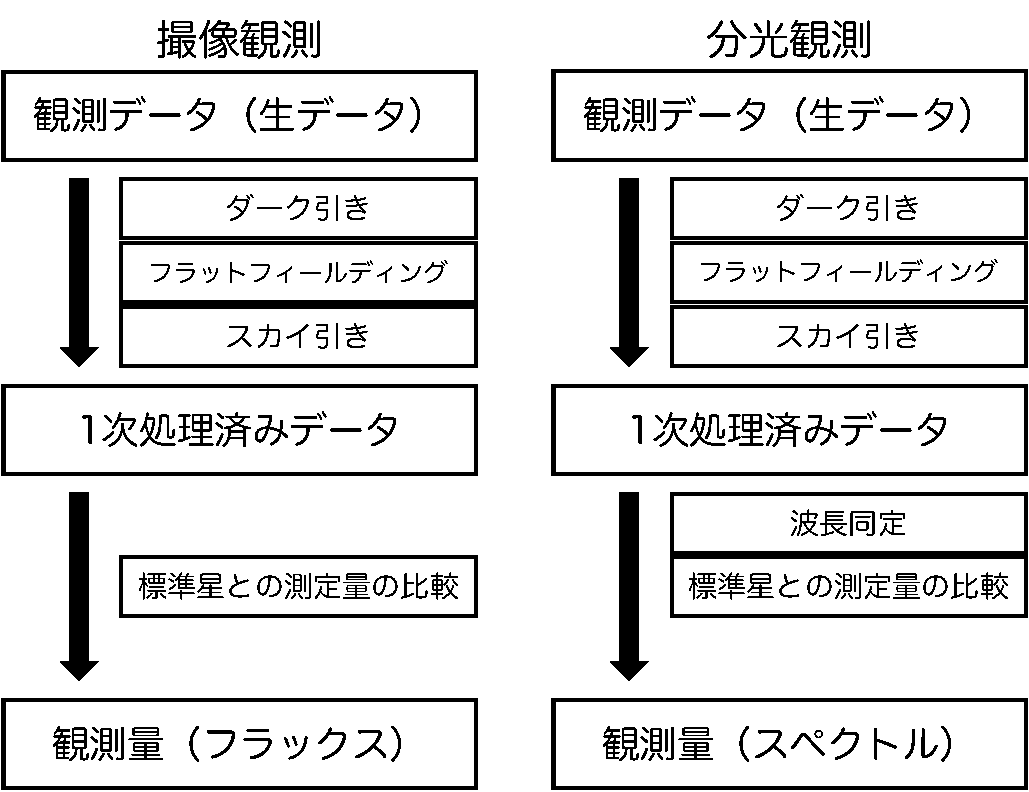
\includegraphics[width=0.7\linewidth]{./fig/chap_5/photo_spec.pdf}
	\caption{撮像/分光観測データの解析の流れ}
  \label{fig:kaiseki_nagare}
\end{figure}
\ref{chap:fandamentals_of_observations}~章の流れに則って得られた観測データのことを、ここでは\textbf{生データ}と呼ぶことにします。生データに自分の欲しい天体からの光だけが入っていれば苦労することはないのですが、\textbf{検出機由来の雑音}や\textbf{夜光}などの影響を受けています。図~\ref{fig:initial_reduction}がそれを模式的に表したものです。
\begin{figure}
  \centering
	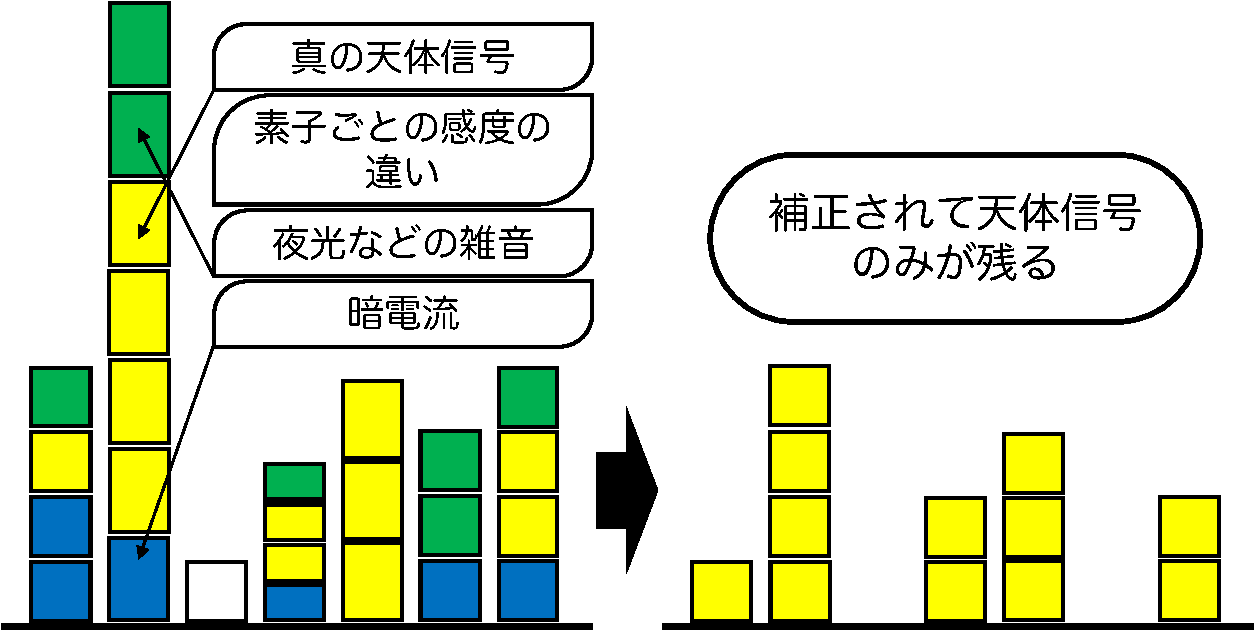
\includegraphics[width=0.7\linewidth]{./fig/chap_5/initial_reduction.pdf}
	\caption[1次処理の仕組み]{1次処理の仕組み。黄色が天体からの光、青が暗電流(ダーク)、緑がスカイ成分を表す。また、大きさの違いは検出機の素子の感度が場所によって異なることを表し、色がついていないのはその素子が死んでいることを表す。このような、観測したい天体のみの情報を使って議論をしたいにも関わらず、混ざってしまう雑音などを取り除く作業が1次処理である。}
  \label{fig:initial_reduction}
\end{figure}
実際に式的にその影響を表すと
\begin{align}
  (\text{生データ}) =  (\text{感度の違い}) \times \left\{  (\text{真の天体信号})+(\text{暗電流})+(夜光などの雑音) \right\}\label{eq:nama_data}
\end{align}
のようになります。\par
\textbf{暗電流}とは、検出機が温度を持っていることで流れてしまう電子雑音のことです。天体放射の検出の仕組みは大まかに
\begin{align*}
  (\text{天体からの光子}) \xrightarrow{\text{検出器}} (\text{光電効果による電子}) \rightarrow (\text{光電流の発生})
\end{align*}
となっています。この二つ目の段階で、天体放射やその他の雑音に加えて、熱雑音による電流が加わります。これを「\textbf{暗電流}」と呼びます。この雑音は単純に検出器を冷やせば減らすことができます。実際、赤外線検出器は$-76\,\mathrm{K}$、市販の可視光の検出器は$-10\,\mathrm{K}$に冷やして使われています。しかし、天体からの放射がわからなくなるほどの雑音の影響を軽減することはできても、完全に$0$にすることは不可能なため、この成分を引く作業が必要となります。この作業を「暗電流」が「\textbf{ダーク}」と呼ばれることから、「\textbf{ダーク引き}」と呼びます。\par
CCDカメラなどの検出機は、多数の素子によって構成されていますが、望遠鏡や、付属する検出器を合わせた系の、光子検出に対する感度は必ずしも一様ではありません。とても強く光子に対して反応する素子も存在する一方で、全く反応しない、「死んだ素子」も存在します。このような感度の違いを補正する処理を\textbf{フラットフィールディング}と呼びます。\par
「\textbf{夜光などの雑音}」とはその名の通り、夜光や大気による雑音の成分です。今回考える主な成分は
\begin{itemize}
  \item 主にKバンドより長い波長で、大気や望遠鏡の熱的な放射成分を見てしまう$(\sim300\,\mathrm{K})$
  \item 主にHバンドで、OH夜光の輝線成分によるフリンジパターン
\end{itemize}
です。これを以降は「\textbf{スカイ}」と呼び、スカイを引く補正のことを、「\textbf{スカイ引き}」と呼ぶことにします。\par
これらの補正のことをまとめて\textbf{1次処理}と呼びます。撮像、分光のどちらでもこの処理が必要になりますが、分光はまとめてIRAFでやってしまった方が楽なので、撮像ではPython、分光ではIRAFを使った処理を行い、観測量を得るにはどうすればよいかをまとめていきます。

\section{撮像データ解析} %%
\label{sect:photo_ana}
今回サンプルとして扱うデータは以下のURLに置いてあります。
\begin{verbatim}
  https://drive.google.com/drive/folders/1ZGkWFySTgc-MVdViP_U_AfD8XPUrSbWi
\end{verbatim}

中身は次のようになっています。
\begin{verbatim}
  dark % ls
  ir0029.fits   ir0030.fits   ir0031.fits   ir0032.fits   ir0033.fits
  flat % ls
  ir0006.fits   ir0007.fits   ir0008.fits   ir0009.fits   ir0010.fits
  raw % ls
  ir0011.fits   ir0012.fits   ir0013.fits   ir0014.fits   ir0015.fits
  ir0016.fits   ir0017.fits   ir0018.fits   ir0019.fits
\end{verbatim}

\section{分光データ解析} %%
\label{sect:spec_ana}